% !TEX TS-program = lualatex
% !TEX encoding = UTF-8 Unicode

\documentclass[]{einformatica}
\usepackage{graphicx} 
\usepackage{soul}
\usepackage{lmodern}
\usepackage{microtype,booktabs}
\usepackage{hyphenat}
\usepackage[all]{nowidow}
\usepackage{tabularx}
\usepackage{floatrow}
\floatsetup[table]{style=plain,capposition=top}
\renewcommand\topfraction{.95}
\renewcommand{\textfraction}{0.05}
\usepackage{xr-hyper}
\usepackage{refcount}
\usepackage[noadjust]{cite}

\usepackage{xcolor}
\usepackage{hyperref}
\hypersetup{
    urlbordercolor = black,
    pdfborderstyle={/S/U/W 1},
}

\usepackage{caption}
\usepackage{lipsum}
\usepackage{cleveref}
%\usepackage{tabu}
\usepackage[newfloat]{minted}
\setminted[R]{breaklines=true,fontsize=\footnotesize,obeytabs=true,tabsize=0}
\setmintedinline[R]{breaklines=true,fontsize=\footnotesize}

\usepackage{listings}
\newenvironment{code}{\captionsetup{type=listing}}{}
\SetupFloatingEnvironment{listing}{name=Listing}

\usepackage[resetlabels,labeled]{multibib}

% Uncomment to include a bibliography of primary studies
% \newcites{S}{List of Primary Studies}

\begin{document}

% Uncomment to include a bibliography of primary studies
% \nociteS{*}

\title{Developer Experience and AI-Agent Contributions: A Large-Scale Study of Usage, Acceptance, and Review Discussion}

\shortauthorshead{Michał Sobczak}

\eIsubmitted{1 Dec. 2025} 
\eIrevised{10 Dec. 2025} 
\eIaccepted{10 Dec. 2025}
\eIpublished{11 Dec. 2024} 

\EIauthorI
   {Michał}
   {Sobczak}
   {University of Warsaw, Poland}
   {ms440009@students.mimuw.edu.pl}
   {0000-1111-2222-3333}
   {*} %  if star present means corresponding author

 
\keywordset{test-driven development, software quality, ...} 

\begin{abstract}[en]
\textbf{Context}:
AI coding agents are increasingly used in public repositories, yet their adoption and outcomes across developer experience levels remain unclear.
\\
\textbf{Objective}:
We examine associations between developer experience and agent-use frequency, acceptance of agent-associated pull requests, and maintainer review discussion.
\\
\textbf{Method}:
We analyzed the AIDev dataset from the MSR 2026 Mining Challenge: $932,791$ pull requests created by $72,189$ users in more than $116,000$ public repositories between December 2024 and August 2025. The data were enriched with GitHub GraphQL activity metrics. After preprocessing and 1\% outlier removal, PCA and (k)-means ($k=3$) grouped $71,467$ developers into activity-based Junior, Mid, and Senior clusters. Differences were tested with Kruskal--Wallis and Bonferroni-corrected Mann--Whitney (U) tests.
\\
\textbf{Results}:
Developers in the Junior cluster used agents significantly less often than those in the Mid and Senior clusters; the latter two did not differ significantly. The Mid cluster had the highest mean acceptance rate (71.55\%, versus 63.33\% for Junior and 67.44\% for Senior), but only the Junior--Mid contrast was significant. Maintainer-comment counts differed significantly between all groups, with Junior receiving the fewest and Mid the most comments, although every group had a median of zero.
\\
\textbf{Conclusions}:
Agent use and contribution outcomes did not follow a simple experience gradient. Comment counts may reflect discussion or task complexity rather than corrections, and the activity-based clusters should not be equated with verified professional seniority.
\end{abstract}

\maketitle 


\section{Introduction}
\subsection*{The evolution of AI tools in programming}
In recent years, the development of artificial intelligence has significantly transformed the software development process. Initially, AI's role was limited to simple browser-based assistants, before evolving toward integration with IDEs in the form of code autocompletion systems. Today we are witnessing another breakthrough: Agents such as \textbf{Claude Code} are gaining access to entire repositories, allowing them not only to fix bugs but also to independently implement new features.

\subsection*{Research objectives}
The main goal of this paper is to investigate the correlation between a developer's level of experience and the way AI tools are used. The analysis attempts to verify whether developers at an early stage of their career path turn to AI agent support more often than experts, and how the acceptance rate of changes within \textit{pull requests} varies depending on the user's level of advancement and the presence of an AI assistant. Additionally, the study examines whether experienced developers can accurately describe a task to an agent so that the generated code requires fewer subsequent corrections.

\subsection*{Dataset}
The research is based on the \textbf{AIDev} \cite{li2025aidev} data set, which is currently the largest and most up-to-date publicly available data set of this type. A key advantage of this data set is that it concerns commercial projects, which significantly increases the reliability of the results in the context of the real job market.

During the initial analysis, I noticed that dividing users into the Junior, Mid, and Senior groups based solely on the data set would not be reliable. Inferring a developer's level of experience solely from their interactions with AI agents could lead to erroneous results. Moreover, the number of \textit{pull requests} created in this dataset exclusively by users is relatively small (6,618 rows compared to the overall total of 932,791 records), which would make a reliable comparison impossible. Therefore, in order to obtain a fuller picture of the studied individuals, I decided to acquire additional external information.

\subsection*{GitHub GraphQL API}
In order to enrich the user profiles, I decided to obtain additional metrics directly from the GitHub platform.
Manually checking so many profiles through a browser would be time-consuming, so I decided to use the GitHub API. Initially I tested the standard REST API, but it quickly turned out that it did not allow extracting sufficiently detailed information, and an additional obstacle was the restrictive hourly request limits. After several experiments, I abandoned this approach in favor of the GitHub GraphQL API. Thanks to lower limits and broader access to data, I was able to efficiently obtain the most important information about the studied group.

For each user, I obtained detailed data including the number of repositories they participated in, and the number of public and private \textit{commits} over the last five years. Additionally, I included statistics on open \textit{pull requests} and reported \textit{issues}. Ultimately, I managed to gather data for 70,486 people out of the entire group of 72,189. Based on this data, I trained a random forest based on decision trees to predict the missing statistics. For this, I used the \textbf{Random Forest Regressor} model, which predicts continuous values for missing users. Numbers of \textit{commits} or \textit{reviews} performed are integers - the result is rounded to whole numbers.

It is worth noting that model validation (an 80/20 split) revealed limited predictive power of the AIDev dataset's features with respect to a user's overall GitHub activity ($R^2$ in the range of 0.05–0.15, and in some cases negative), suggesting that both data sources describe partially different aspects of activity, and the values imputed for missing users should be treated with some caution.

\section{Related work\label{sec:intro}}
\section{Methodology}\label{sec:method}

Analizowaliśmy nie tylko kod, ale również powiązane z nim metadane. Proces badawczy składał się z czterech etapów: wyboru wersji AIDev, wzbogacenia profili deweloperów o dane aktywności z GitHub, podziału użytkowników na grupy oraz porównania korzystania z agentów pomiędzy tymi grupami. Wyniki na poziomie pull requestów zostały zagregowane per programista, by uniknąć traktowania wielu wkładów tej samej osoby jako niezależnych obserwacji.

\subsection{Data sources and sample construction}

Korzystamy z wydania Zenodo v3 zbioru AIDev (DOI \texttt{10.5281/zenodo.16919272}), opisanego w Sekcji 1.

Aktywność w AIDev opisuje deweloperów głównie w odniesieniu do wkładu powiązanego z agentami. Aby uzyskać szerszy zakres informacji, wzbogaciliśmy rekordy za pomocą GitHub GraphQL API. Tabela~\ref{tab:profile-indicators} przedstawia 12 ilościowych wskaźników użytych do klastrowania. Wskaźniki pięcioletnie obejmują pięć lat poprzedzających zbieranie danych. GitHub udostępnia tylko zagregowaną liczbę kontrybucji do prywatnych repozytoriów (nie tylko commitów, i tylko dla użytkowników, którzy zgodzili się to pokazywać) - nie należy tego interpretować jako dokładną liczbę prywatnych commitów. W procesie gromadzenia danych login uznawano za niedostępny - usunięty, przemianowany lub z jakiegoś innego powodu niedostępny - gdy API zwróciło status inny niż 200. Odpowiadający im deweloperzy to dokładnie ci, których wskaźniki później oszacowano metodą lasu losowego, opisaną poniżej. Zbieranie danych GraphQL przeprowadzono 6 maja 2026 roku. Należy zwrócić uwagę, że jest to około 9 miesięcy po okresie, którego dotyczą dane z AIDev, i mogły one ulec zmianie w tym czasie.

Zbieranie danych GraphQL dało rekordy aktywności dla 70\,434 z 72\,189 deweloperów (97,57\%). Wskaźniki liczbowe pozostałych 1755 deweloperów oszacowano za pomocą modeli regresji lasu losowego \cite{breiman2001random}. Modele oceniono przy podziale 80/20 na zbiór treningowy i testowy, a przewidziane wartości liczbowe zaokrąglano do liczb całkowitych. Ich skuteczność predykcyjna była ograniczona - obserwowane wartości $R^2$ przedstawia Tabela~\ref{tab:r2-values}. Wartości te należy więc traktować jako przybliżone uzupełnienie brakujących profili, a nie wiarygodną rekonstrukcję ich aktywności.

\begin{table}[tb]
    \centering
    \caption{Skuteczność predykcyjna ($R^2$) modeli imputacji lasem losowym.}
    \label{tab:r2-values}
    \small
    \begin{tabular}{lr}
        \toprule
        \textbf{Wskaźnik} & \textbf{$R^2$} \\
        \midrule
        \texttt{collab\_breadth} & 0,098 \\
        \texttt{5yr\_prs\_opened} & 0,088 \\
        \texttt{5yr\_reviews\_given} & 0,020 \\
        \texttt{5yr\_public\_commits} & $-0{,}073$ \\
        \texttt{5yr\_private\_work} & $-0{,}272$ \\
        \bottomrule
    \end{tabular}
\end{table}
\begin{table}[tb]
    \centering
    \caption{Wskaźniki użyte do wyznaczenia profili aktywności deweloperów.}
    \label{tab:profile-indicators}
    \small
    \begin{tabularx}{\linewidth}{@{}p{0.31\linewidth}X@{}}
        \toprule
        \textbf{Wskaźnik} & \textbf{Operacjonalizacja} \\
        \midrule
        Zakres współpracy & Liczba repozytoriów, do których deweloper wniósł wkład. \\
        Publiczne commity & Publiczne kontrybucje typu commit w ciągu poprzedzających pięciu lat. \\
        Aktywność zastrzeżona & Zastrzeżone kontrybucje w ciągu poprzedzających pięciu lat, gdy ujawnione przez GitHub. \\
        Otwarte pull requesty & Pull requesty otwarte w ciągu poprzedzających pięciu lat. \\
        Złożone recenzje & Recenzje pull requestów złożone w ciągu poprzedzających pięciu lat. \\
        Staż konta & Czas, jaki upłynął od utworzenia konta GitHub. \\
        Obserwujący & Liczba obserwujących w momencie zbierania danych. \\
        Maksymalna liczba gwiazdek & Największa liczba gwiazdek wśród repozytoriów należących do dewelopera. \\
        Maksymalna liczba forków & Największa liczba forków wśród repozytoriów należących do dewelopera. \\
        Rozpiętość aktywności Agentic-PR & Liczba dni między pierwszym a ostatnim Agentic-PR dewelopera. \\
        Różnorodność agentów & Liczba różnych agentów kodujących użytych w Agentic-PR dewelopera. \\
        Zakres repozytoriów Agentic-PR & Liczba różnych repozytoriów, w których deweloper ma Agentic-PR. \\
        \bottomrule
    \end{tabularx}
\end{table}

\subsection{Preprocessing and activity-profile construction}

Wskaźniki były silnie prawoskośne i różniły się o kilka rzędów wielkości. Zastosowaliśmy transformację log(1+x), a następnie wystandaryzowaliśmy każdą cechę do średniej zero i wariancji jeden. Następnie użyliśmy Isolation Forest z parametrem kontaminacji ustawionym na 1\%, aby usunąć najbardziej skrajne przypadki \cite{liu2008isolation}. W wyniku tej procedury usunięto 722 programistów, pozostawiając 71\,467 profili do głównej analizy.

Transformację kwantylową w kierunku rozkładu normalnego brzegowego wypróbowano najpierw zamiast log(1+x), ale kontrola wrażliwości typu complete-case (Sekcja 5) wykazała jej niestabilność. Klastrowanie na danych zawierających wyłącznie deweloperów z rzeczywistymi danymi GraphQL zgadzało się z klastrowaniem pełnej populacji jedynie przy Adjusted Rand Index = 0,46. Ta sama kontrola z log(1+x) dała Adjusted Rand Index = 0,98, więc pozostano przy tej drugiej metodzie.

Analizę głównych składowych obliczono na przekształconych wskaźnikach, aby wspomóc interpretację dominujących osi zmienności, a nie jako etap redukcji wymiarowości zasilający algorytm klastrowania \cite{jolliffe2016principal}. Pierwsze dwie główne składowe zachowują jedynie około 50\% wariancji, więc projekcja do 2 wymiarów odrzucałaby mniej więcej połowę informacji. Dlatego klastrowanie przeprowadziliśmy na pełnej, 12-wymiarowej, oczyszczonej reprezentacji; PCA(2) raportujemy osobno, wyłącznie w celu wizualizacji, które wskaźniki napędzają dwie dominujące osie. Jak pokazuje Rysunek~\ref{fig:pca-loadings}, pierwsza składowa ładuje się dodatnio na wskaźnikach aktywności i można ją interpretować jako oś ogólnej aktywności. Druga składowa przeciwstawia aktywność powiązaną z agentami i wielkość wkładu publicznego ogólnej rozpoznawalności oraz aktywności recenzenckiej.

\begin{figure}[tb]
    \centering
    
\includegraphics[width=0.92\linewidth]{pca_1.png}
    \vspace{0.5em}
    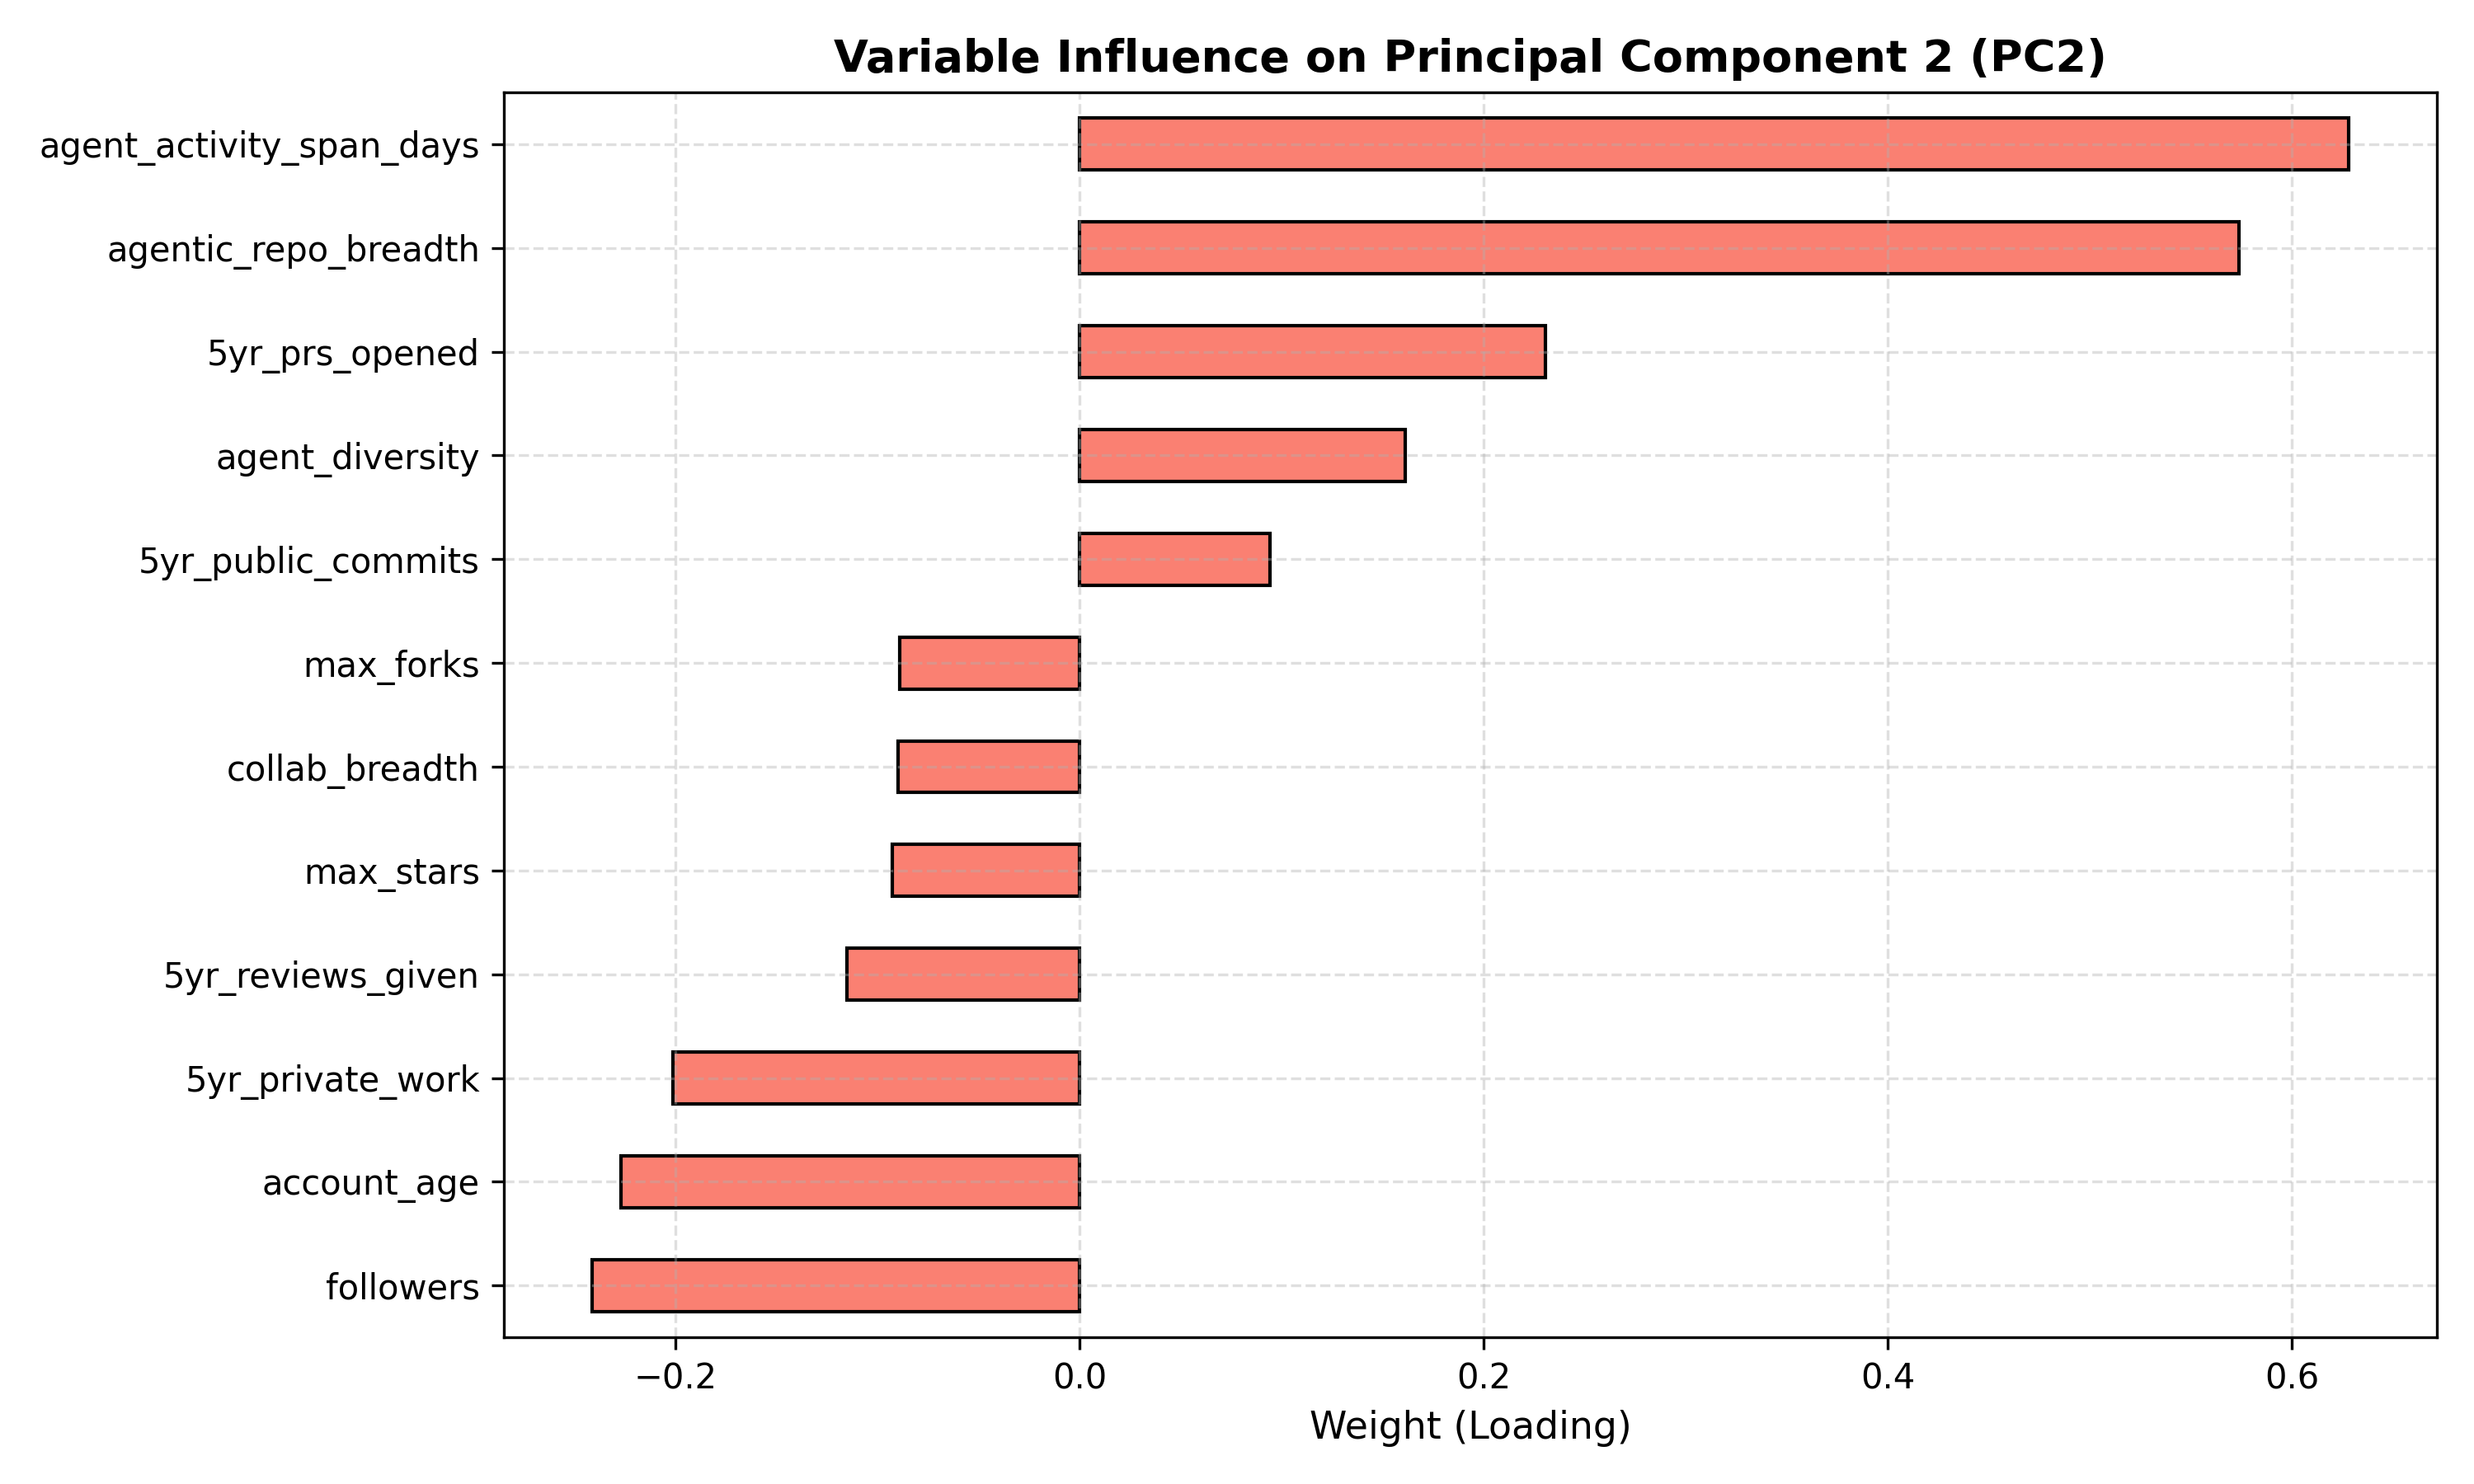
\includegraphics[width=0.92\linewidth]{pca_2.png}
    \caption{Ładunki wskaźników aktywności na dwóch dominujących osiach zmienności (PC1, PC2), obliczone wyłącznie w celach interpretacyjnych; PC1+PC2 zachowują około 50\% wariancji i nie są używane jako dane wejściowe do klastrowania. PC1 reprezentuje przede wszystkim ogólną aktywność na GitHub, podczas gdy PC2 przeciwstawia aktywność powiązaną z agentem i wielkość wkładu publicznego ogólnej rozpoznawalności i aktywności recenzenckiej.}
    \label{fig:pca-loadings}
\end{figure}

Pełną, 12-wymiarową, oczyszczoną reprezentację podzieliliśmy za pomocą klastrowania $k$-średnich \cite{lloyd1982least}. Zbadaliśmy również rezultaty dla różnych wartości $k=2,\ldots,10$ przy użyciu average silhouette width \cite{rousseeuw1987silhouettes} oraz gap statistic \cite{tibshirani2001gap}, obliczonych na tej samej 12-wymiarowej reprezentacji. Rysunek~\ref{fig:cluster-diagnostics} pokazuje, że $k=3$ nie jest optimum liczbowym według żadnej z tych statystyk. Mimo to zachowaliśmy $k=3$ jako celowo uproszczony i interpretowalny parametr, dopasowany do porównań pomiędzy profilami o niskiej, pośredniej i wysokiej aktywności. Analiza jest więc warunkowa względem tego wyboru i nie zakłada, że trzy klastry stanowią wewnętrzną strukturę populacji deweloperów.

\begin{figure}[tb]
    \centering
    
\includegraphics[width=0.90\linewidth]{silnouette.png}
    \vspace{0.5em}
    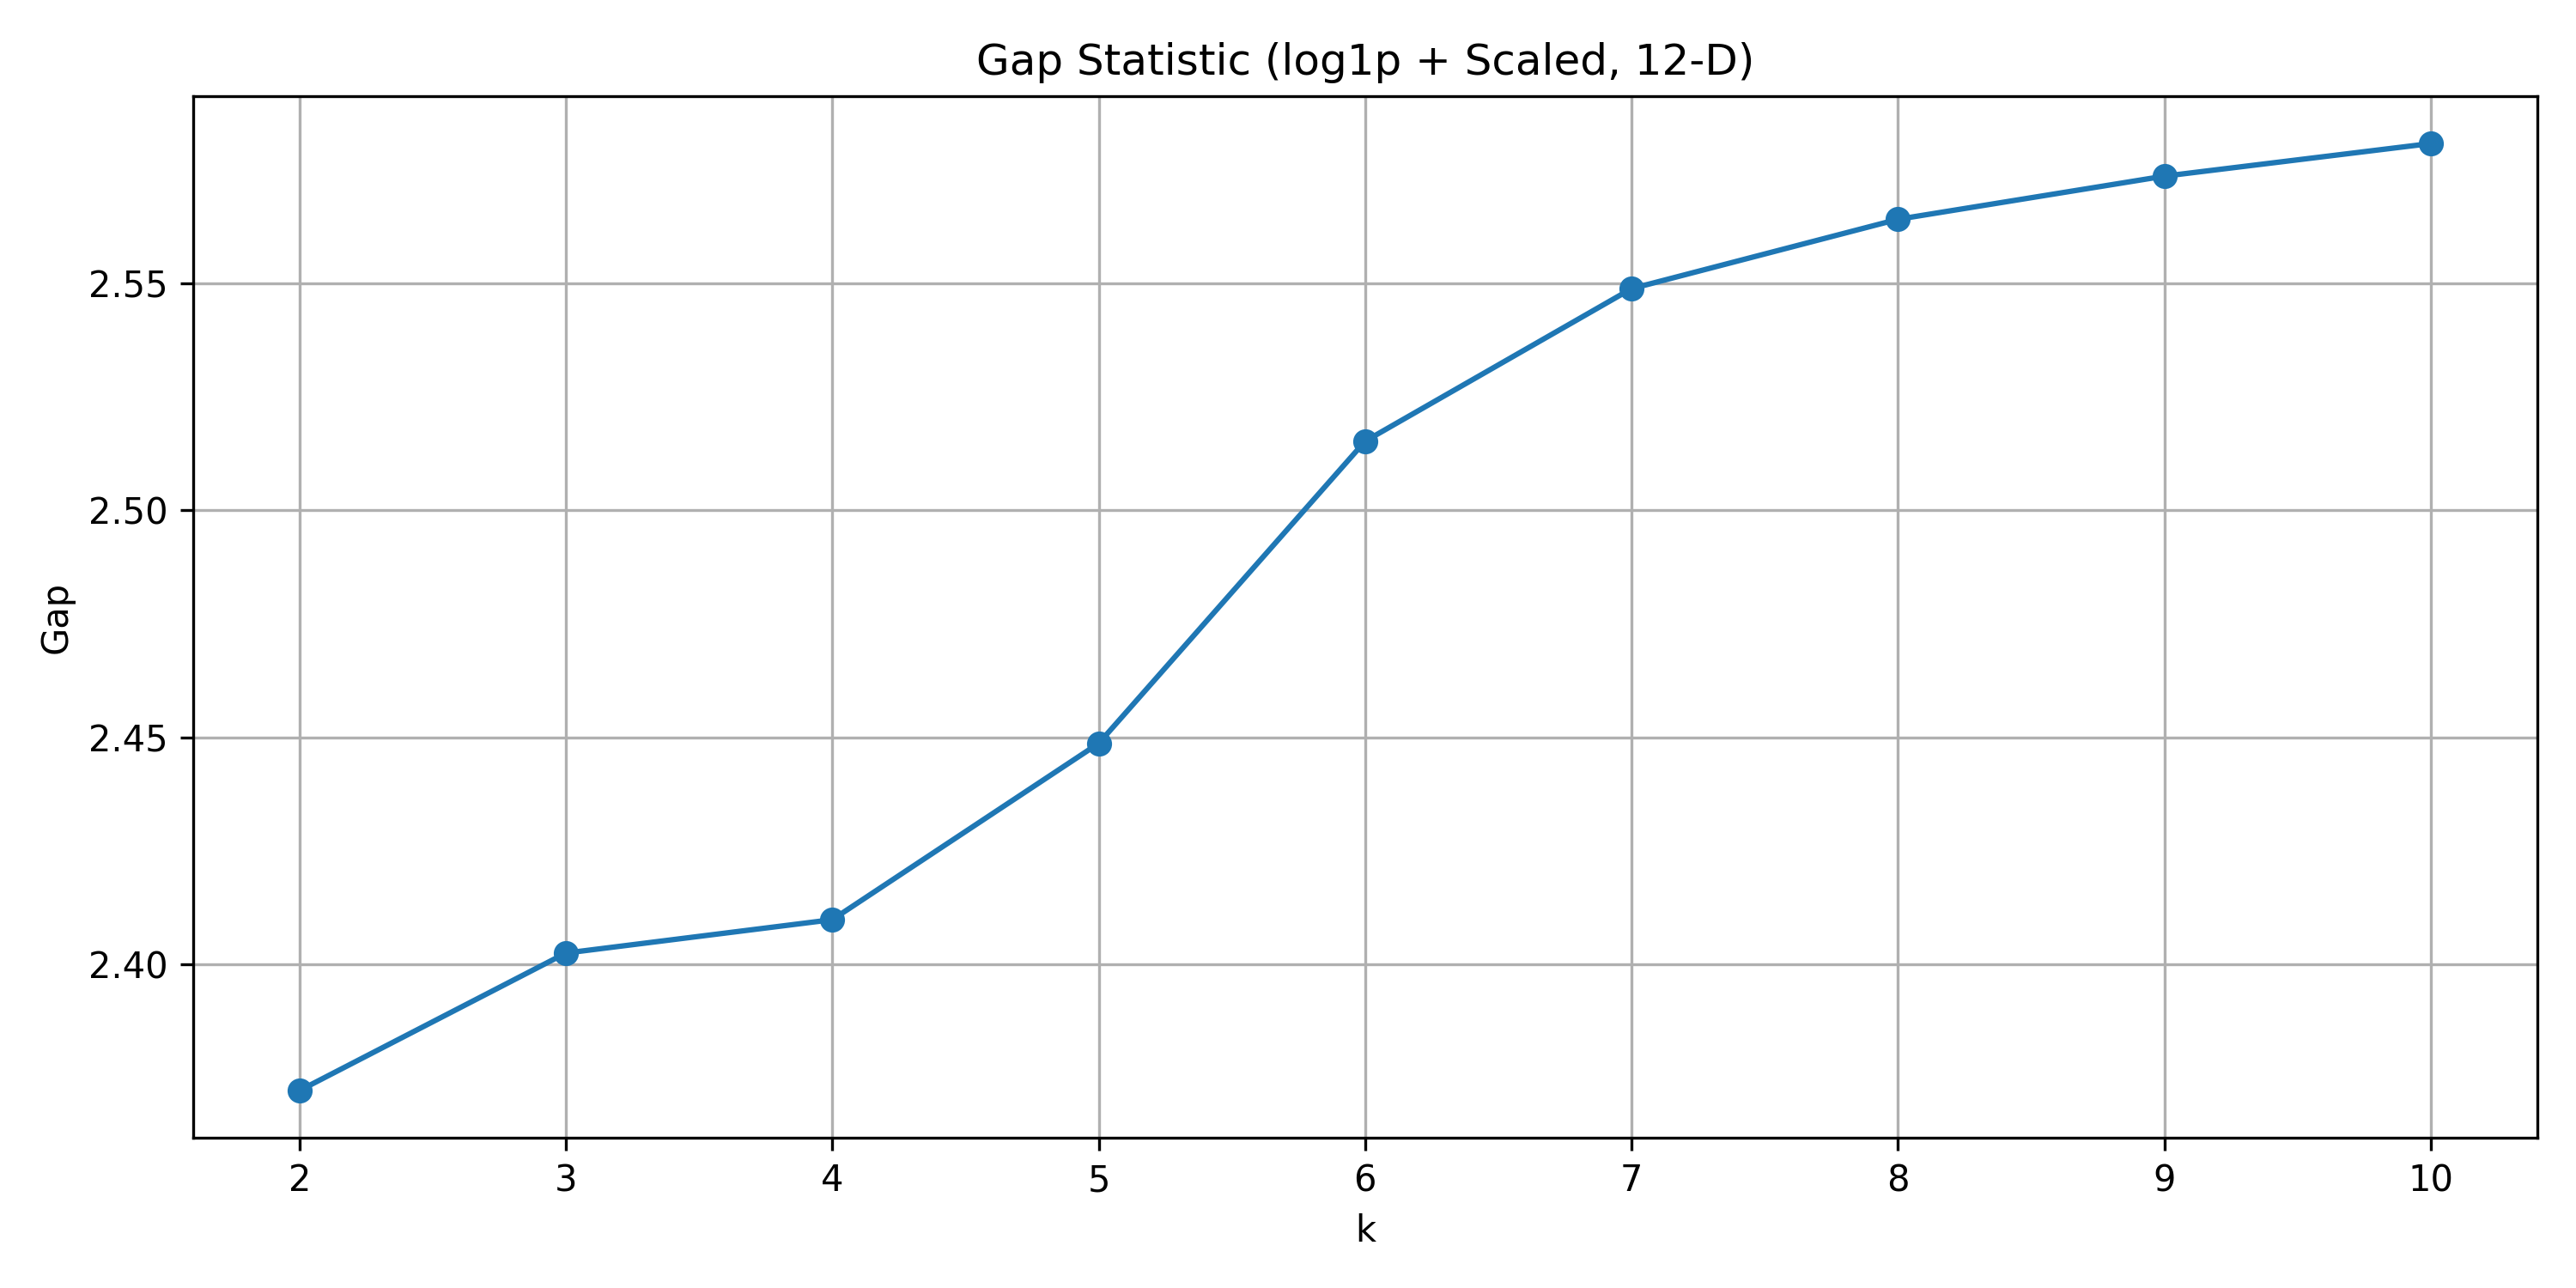
\includegraphics[width=0.90\linewidth]{gap_statistic.png}
    \caption{Diagnostyki szerokości sylwetki i statystyki luki dla kandydujących wartości $k$, obliczone na 12-wymiarowych danych wejściowych klastrowania. $k=3$ nie jest optimum liczbowym według żadnej z diagnostyk; jest zachowane jako wybór projektowy podyktowany interpretowalnością.}
    \label{fig:cluster-diagnostics}
\end{figure}

Dla czytelności profile o niskiej, pośredniej i wysokiej aktywności nazywamy odpowiednio \emph{Junior}, \emph{Mid} i \emph{Senior}. Liczą one odpowiednio 44\,854, 12\,705 i 13\,908 deweloperów. Te etykiety nie są zweryfikowanymi stanowiskami zawodowymi, etapami kariery ani bezpośrednimi pomiarami kompetencji programistycznych. Ta rozbieżność ma konkretne znaczenie dla RQ1: profil Mid okazuje się mieć najwyższą medianę liczby Agentic-PR spośród trzech profili (Sekcja~\ref{sec:results}), mimo że w rankingu złożonego wyniku aktywności plasuje się niżej niż Senior, ponieważ ten wynik odzwierciedla też wskaźniki (obserwujący, staż konta, gwiazdki i forki repozytoriów), na których Senior wypada wyżej.

\subsection{Outcome measures}

Zmienne wynikowe nie były uwzględnione wśród danych wejściowych klastrowania.

\paragraph{RQ1: AI-agent use intensity.}
Dla każdego dewelopera policzyliśmy liczbę Agentic-PR powiązanych z tym deweloperem w pełnym zbiorze danych AIDev. Zmienna ta mierzy obserwowaną wielkość wkładu w oknie czasowym zbioru danych. Nie mierzy natomiast udziału całkowitej pracy dewelopera wykonanej z użyciem agenta ani ogólnego prawdopodobieństwa, że deweloper korzysta z narzędzi AI.

\paragraph{RQ2: pull-request acceptance.}
Dla każdego dewelopera obliczyliśmy proporcję rozstrzygniętych Agentic-PR, które zostały scalone. Pull request klasyfikowano jako scalony, gdy jego pole \texttt{merged\_at} było niepuste, a jako odrzucony, gdy został zamknięty bez scalenia. Otwarte pull requesty wykluczono z mianownika, zamiast traktować je jako odrzucone. Deweloperów bez rozstrzygniętego Agentic-PR wykluczono z tej analizy. Ten wynik dotyczy akceptacji pull requestów, a nie poprawności poszczególnych wygenerowanych linii kodu ani ogólnej jego jakości.

\paragraph{RQ3: Agentic-PR acceptance vs.\ a human-authored baseline.}
AIDev osobno udostępnia tabelę \texttt{human\_pull\_request} - bazową próbę pull requestów autorstwa ludzi (bez udziału agenta), pochodzącą z repozytoriów z ponad 500 gwiazdkami. Rozważaliśmy początkowo programistów znajdujących się w obu tych grupach, ale okazało się, że jedynie 351 z 2515 odrębnych autorów w \texttt{human\_pull\_request} znalazło się jednocześnie wśród 72\,189 deweloperów powiązanych z Agentic-PR. Stąd decyzja, że w RQ3 porównujemy dwie niezależne populacje: wskaźnik akceptacji wszystkich Agentic-PR, zsumowany po profilach aktywności, w porównaniu do wskaźnika akceptacji \texttt{human\_pull\_request}, przy użyciu tej samej klasyfikacji scalony/odrzucony/otwarty co w RQ2. Jest to porównanie na poziomie populacji, a nie dopasowane na poziomie deweloperów, a bazowa populacja jest sama w sobie ograniczona do węższej próby repozytoriów niż pełna populacja Agentic-PR.

\subsection{Statistical analysis}
Rozkłady zmiennych wynikowych nie dało się prosto porównać z popularnymi i znanymi rozkładami, a miary oparte na liczności zawierały wiele remisów oraz zer. Dla RQ1-RQ2, z których każde porównuje trzy profile aktywności, najpierw stosujemy test Kruskala-Wallisa, aby ocenić, czy rozkłady wyniku różnią się pomiędzy trzema grupami. Istotny wynik testu ogólnego jest uzupełniany dwustronnymi parami testów Manna-Whitneya $U$, przy czym trzy porównania parami dla każdego pytania badawczego korygujemy poprawką Bonferroniego, przy poziomie istotności $\alpha=0,05$. RQ3 porównuje tylko dwie niezależne grupy, więc stosujemy pojedynczy test Manna-Whitneya $U$, bez etapu testu ogólnego Kruskala-Wallisa i bez poprawki Bonferroniego.

Dla każdej grupy zanotowaliśmy liczność próby, średnią, odchylenie standardowe i medianę. Dodatkowo uzupełniamy wartości $p$ wielkościami efektu: epsilon-kwadrat dla testu Kruskala-Wallisa oraz korelacją rangowo-biseryjną dla porównań parami. Każdą wielkość efektu raportujemy wraz z 95\% przedziałem ufności uzyskanym metodą nieparametrycznego bootstrapu: dla epsilon-kwadrat losujemy ponownie każdą grupę niezależnie ze zwracaniem, przeliczamy statystykę Kruskala-Wallisa i bierzemy 2,5. oraz 97,5. percentyl z 2000 powtórzeń losowania. Ta sama procedura, zastosowana do dwóch porównywanych grup, jest używana dla każdej korelacji rangowo-biseryjnej w porównaniach parami. Wszystkie analizy dotyczą związków pomiędzy profilami opartymi na aktywności a obserwowanymi wynikami.

\section{Results\label{sec:results}}

\subsection{How does a developer's experience correlate with the frequency of using AI agents?}

In order to assess the relationship between developers' level of experience and the frequency of using AI agents, a nonparametric Kruskal-Wallis test and post-hoc Mann-Whitney tests with Bonferroni correction were performed.

The Kruskal-Wallis test showed a statistically significant difference in the frequency of generating \textit{pull requests} between the analyzed experience groups.

The post-hoc analysis showed the following relationships:
\begin{itemize}
    \item The \textbf{Junior} group is characterized by a significantly lower frequency of using AI agents compared to the other groups.
    \item No statistically significant differences were found between the \textbf{Mid} and \textbf{Senior} groups.
\end{itemize}

Developers at the \textbf{Mid} and \textbf{Senior} level use AI agents the most, achieving the highest median usage.

\begin{figure}[H]
    \centering
    
\includegraphics[width=0.85\linewidth]{summary.png}
    \label{fig:summary-exp1}
\end{figure}

\begin{figure}[H]
    \centering
    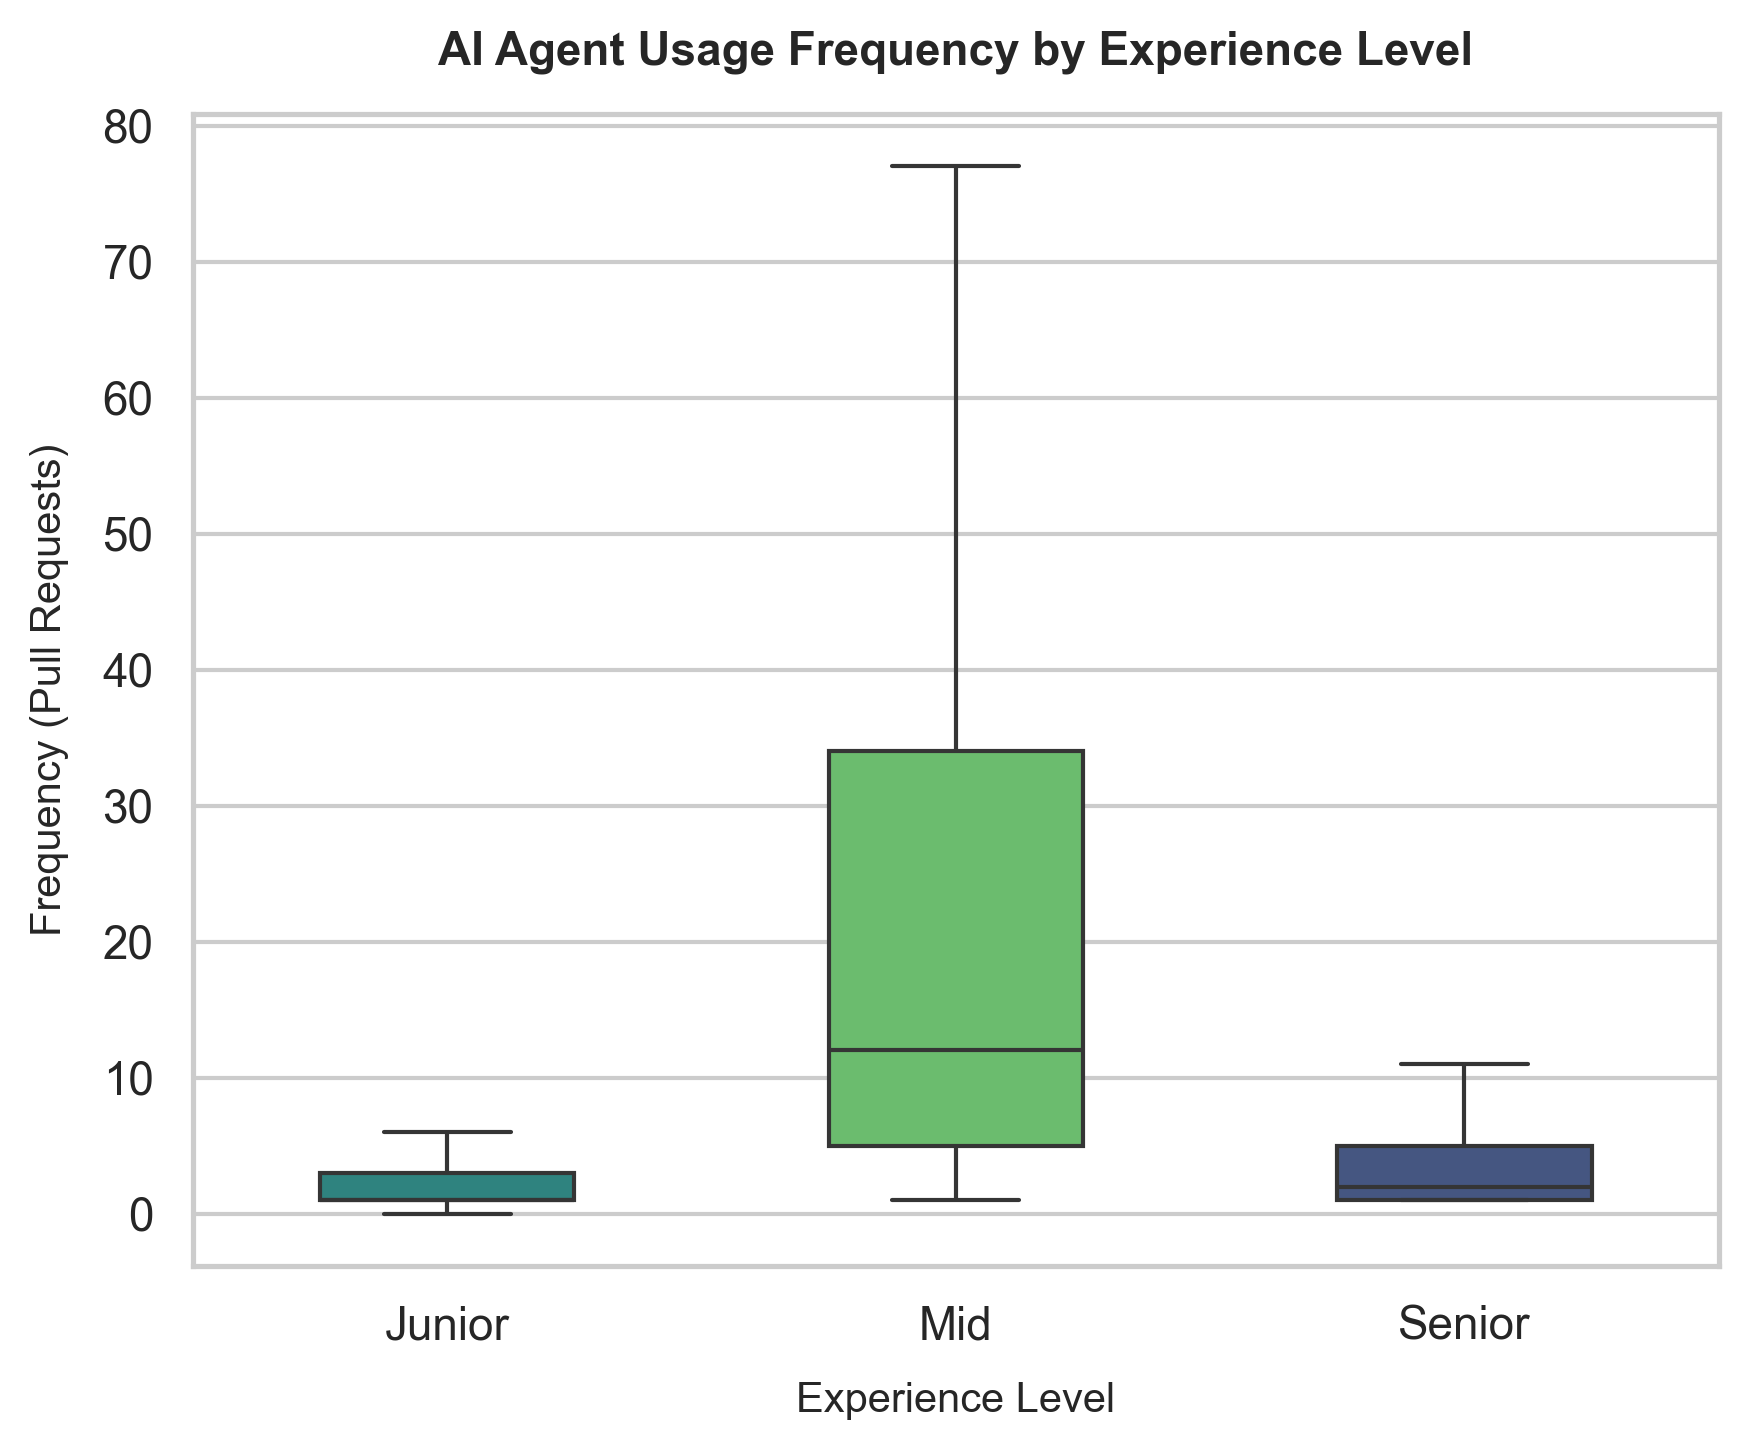
\includegraphics[width=0.85\linewidth]{box_plot.png}
    \label{fig:box_plot-exp1}
\end{figure}

\subsection{Does human experience translate into a higher acceptance rate of agent-generated code?}


The analysis performed shows that a developer's level of experience affects the acceptance rate of code generated by AI agents. The Kruskal-Wallis test confirmed the existence of significant differences between the studied groups. A detailed analysis using post-hoc tests (Mann-Whitney U with Bonferroni correction) reveals the following relationships:

\begin{itemize}
    \item Developers at the \textbf{Mid} level achieve the highest average code acceptance rate as well as the highest median. 
    
    \item Code generated by \textbf{Seniors} shows a lower median acceptance rate among the other groups, but the tests did not show significant differences between the remaining groups ($p=0.43$ for \textbf{Juniors} and $p = 1.00$ for \textbf{Mids})
\end{itemize}

Based on the data, it can be concluded that human experience does not automatically translate into a higher code acceptance rate. Developers at the \textbf{Mid} level show the greatest effectiveness in accepting AI agent proposals.

\begin{figure}[H]
    \centering
    
\includegraphics[width=1\linewidth]{second_experiment_box_plot.png}
    \label{fig:boxplot-exp2}
\end{figure}
 \begin{figure}[H]
     \centering
     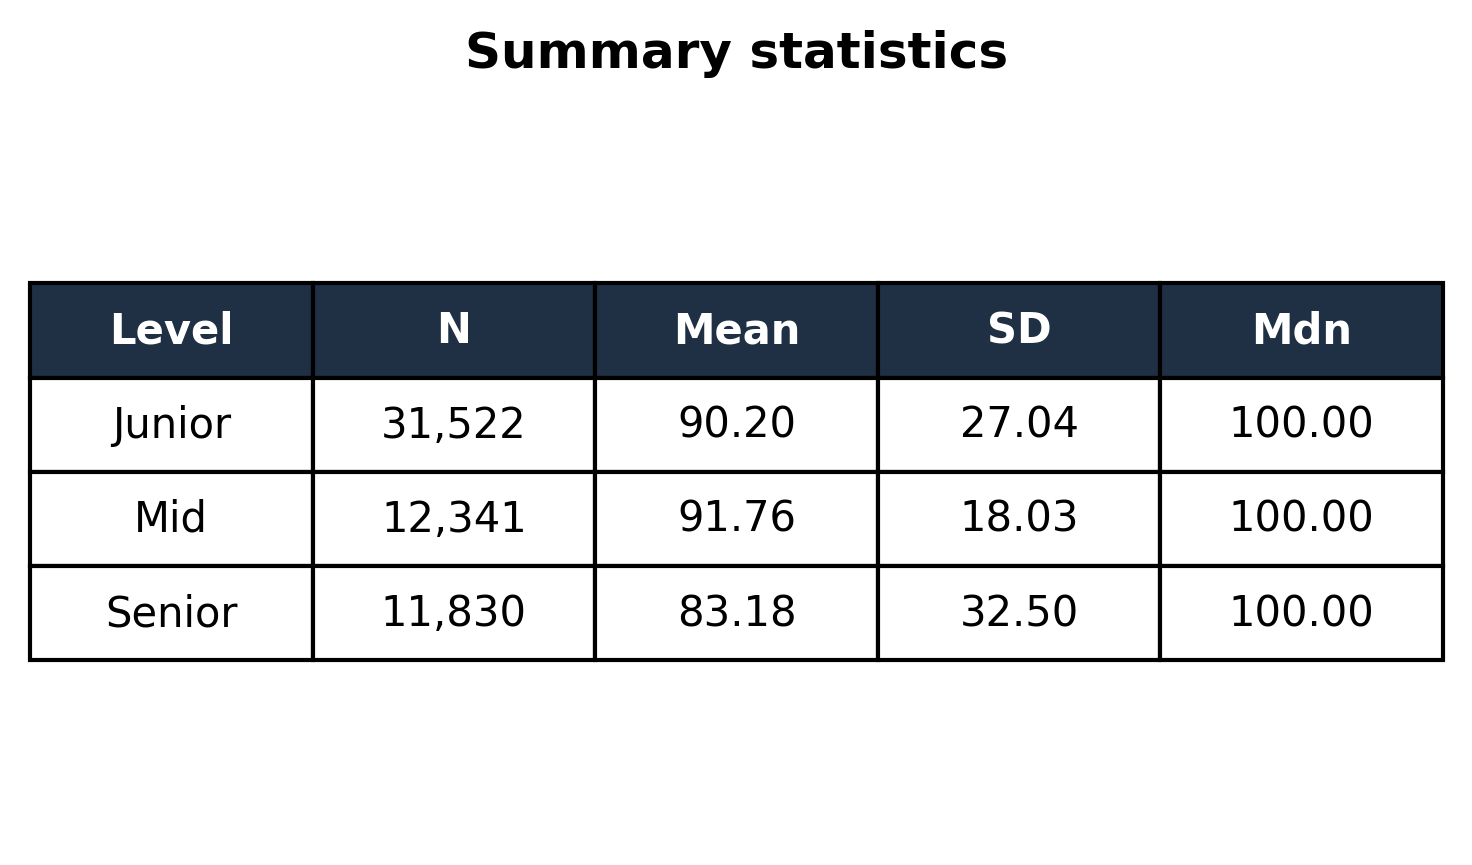
\includegraphics[width=1\linewidth]{second_boxplot.png}
     \label{fig:summary-exp2}
 \end{figure}


\subsection{Do changes introduced by the junior group using AI require more corrections (measured by the number of comments) from the project maintainer?}
The analysis was based on counting comments left by maintainers within \textit{pull requests}. In cases where the author of a \textit{pull request} turned out to be a bot, the associated \textit{issue} was checked, and its creator was treated as the actual author of the changes.

To verify this hypothesis, the \textbf{Kruskal-Wallis} test was used (robust to a large number of zero values in the data). The test confirmed the existence of statistical differences between all groups. Analysis using Mann-Whitney tests with Bonferroni correction showed that the differences are significant at every level of comparison:
\begin{itemize}
    \item \textbf{Junior} vs \textbf{Mid}: $p < 0.001$ 
    \item \textbf{Junior} vs \textbf{Senior}: $p < 0.001$ 
    \item \textbf{Mid} vs \textbf{Senior} $p < 0.001$
\end{itemize}

Code generated or supported by AI in the case of Juniors produced the lowest average number of comments. The highest rate was recorded in the \textbf{Mid} group. This result is somewhat surprising in the context of the hypothesis posed, and may result from the fact that Juniors create relatively simpler \textit{pull requests}, while Mids undertake more complex changes that generate more remarks from maintainers - not necessarily due to lower code quality.

\begin{figure}[H]
    \centering
    
\includegraphics[width=1\linewidth]{third_experiment_table.png}
    \label{fig:table-exp3}
\end{figure}

\begin{figure}[H]
    \centering
    
\includegraphics[width=1\linewidth]{third_experiment.png}
    \label{fig:boxplot-exp3}
\end{figure}

\section{Threats to validity\label{sec:threats}}

\paragraph{Construct validity.}
\emph{Junior}, \emph{Mid}, and \emph{Senior} are unsupervised clusters over observable GitHub activity, not verified job titles or measured skill; a developer's placement reflects relative activity within the analyzed population, not a career stage. Three of the twelve clustering indicators -- Agentic-PR activity span, agent diversity, and Agentic-PR repository breadth -- directly describe agent-associated activity rather than independent, pre-agent experience, so the profiles are partly constructed from the same kind of behavior RQ1 and RQ2 later measure; the remaining nine (GraphQL-derived contribution history, plus followers, account tenure, and repository stars/forks) describe general GitHub activity not tied to agent use. The RQ3 outcome counts non-bot comments from any other account, not comments verified to come from a maintainer; it is best read as a proxy for visible discussion volume, not review effort or defect count. Bot and agent detection relies on AIDev's own labeling and simple login-pattern filtering, which may miscount atypically named bot or human accounts. The GraphQL profile enrichment was collected on 6 May 2026, about nine months after AIDev's own 1 August 2025 cutoff; indicators such as followers, account tenure, and yearly contribution counts reflect each account's state at the later collection date, not at the time of its Agentic-PRs, so part of the activity profile may postdate the contributions it is meant to characterize.

\paragraph{Internal validity.}
The design is observational: none of the four research questions supports a causal claim about the effect of experience or of agent use. PR complexity, task type, and repository governance norms are not controlled for and plausibly confound both acceptance rate and comment volume; RQ2's finding that acceptance decreases with activity level, for instance, is also consistent with more active developers attempting more difficult tasks rather than with agents serving them less well. The $k=3$ operationalization was retained for interpretability even though neither silhouette width nor the gap statistic identifies it as the strict numerical optimum (Section~\ref{sec:method}); a different $k$ or a different clustering algorithm could yield different group compositions and, in turn, different outcome comparisons. The 1,755 developers with GraphQL-imputed indicators were estimated from AIDev-derived features with weak explanatory power (observed $R^2$ between $-0.27$ and $0.10$, Section~\ref{sec:method}); their placement into activity profiles is comparatively uncertain.

A complete-case sensitivity check -- clustering only the 70,434 developers with real, non-imputed GraphQL data, instead of the full 72,189 -- initially found a quantile-transformation-based version of the pipeline in Section~\ref{sec:method} to be unstable under this population change: cluster assignment agreed with the full-population clustering, for the same overlapping developers, at only Adjusted Rand Index $=0.46$, and RQ1's and RQ2's Junior-vs-Mid ordering reversed. We traced this to the quantile transformation step: because several indicators are heavily zero-inflated, quantile transformation maps values by rank within the current sample, so removing even a small fraction of the population shifts those ranks for everyone else. Re-running the same complete-case comparison with $\log(1+x)$ transformation followed by standardization in place of quantile transformation gave Adjusted Rand Index $=0.98$, essentially stable, which is why $\log(1+x)$ plus standardization -- not quantile transformation -- is the preprocessing step used throughout this paper (Section~\ref{sec:method}).

We also reran RQ1--RQ3 restricted to the 70,434 complete-case developers under the now-adopted $\log(1+x)$ pipeline (RQ4 does not depend on clustering and is unaffected). RQ1 and RQ2 were essentially unchanged (e.g.\ RQ1: Junior/Mid/Senior means $3.59/42.27/7.18$ vs.\ $3.57/42.12/7.94$ in the full-population analysis; RQ2: $90.3\%/91.8\%/83.4\%$ vs.\ $90.2\%/91.8\%/83.2\%$), with the same pairwise significance pattern in both cases. \textbf{RQ3 did not replicate}: under the complete-case restriction its already-small AIDev-pop sample shrinks further and shifts composition (Senior drops from 13,434 to 4,366 observations), the mean ordering reverses (Junior $0.45$, Mid $0.56$, Senior $0.73$, i.e.\ increasing rather than decreasing with activity level), and the Kruskal--Wallis test is no longer significant ($p=0.77$). RQ3 is therefore the least robust of the four research questions: its direction and significance both depend on whether the 1,755 imputed developers are included, on top of the small-sample concerns already noted below.

We additionally ran four further sensitivity checks against the $\log(1+x)$-based pipeline. (i) \emph{Alternative $k$}: at $k=4$ and $k=5$, the three main clusters remain close to their $k=3$ sizes, with the additional clusters carved out of Senior as small, higher-activity splinters, rather than a wholesale reorganization. (ii) \emph{Repeated initializations}: rerunning the full pipeline (Isolation Forest and $k$-means) with five different random seeds gave Adjusted Rand Index between $0.98$ and $0.99$ against the reported clustering -- highly stable. (iii) \emph{Retained outliers}: skipping Isolation Forest entirely gives Adjusted Rand Index $=0.64$ against the reported clustering, driven almost entirely by the Senior profile, which shrinks from 13,908 to 1,586 developers as the most extreme profiles get isolated into their own cluster instead of being excluded beforehand; Junior and Mid are comparatively stable. (iv) \emph{Excluding the AIDev-derived indicators} (Agentic-PR activity span, agent diversity, and repository breadth), leaving only the nine remaining indicators: this is the least stable of the four checks, Adjusted Rand Index $=0.32$, and cluster sizes shift substantially (Mid grows from 12,705 to 28,329). We re-ran RQ1 and RQ2 under this 9-indicator clustering: RQ2's qualitative finding holds -- Senior still has the lowest acceptance rate (80.7\% vs.\ 90.4\% Junior and 90.2\% Mid) -- but RQ1's Mid-vs-Senior contrast is much weaker (Agentic-PR means 17.6 vs.\ 20.8, close to reversing) than under the full 12-indicator clustering, consistent with the construct-validity concern raised above: part of RQ1's large effect size is attributable to the clustering itself being partly built from agent-usage indicators.

\paragraph{External validity.}
The dataset covers Agentic-PRs from five specific coding agents on public GitHub repositories up to 1 August 2025, an early period of agent adoption; usage patterns, acceptance norms, and maintainer behavior around agent-generated code may shift as the tooling and community norms mature, so the reported associations should not be extrapolated to later periods or to private/enterprise repositories without re-verification. RQ3 and RQ4 are further restricted to AIDev-pop and to a $>500$-star baseline respectively, because richer interaction data (comments, reviews, commits, issues) and the human-authored comparison sample were collected by AIDev's authors only for repositories above those popularity thresholds; both results describe high-visibility, high-star repositories specifically and may not generalize to the long tail of smaller projects that make up most of the full-scope population.

\paragraph{Conclusion validity.}
The outcome distributions are strongly non-normal and zero-inflated, which motivated the nonparametric tests and the Bonferroni correction used throughout (Section~\ref{sec:method}). With sample sizes in the tens of thousands, very small differences can reach statistical significance regardless of practical importance; this applies most clearly to RQ2 ($\varepsilon^2=0.043$) and especially RQ3 ($\varepsilon^2=0.009$), whose effect sizes are small even though their $p$-values are not. RQ1 is an exception: its effect size ($\varepsilon^2=0.32$) is large by conventional standards, so its significance reflects a substantial association, not only a large sample. RQ3 and RQ4 additionally rest on markedly unequal group sizes (RQ3's Junior profile has only 187 observations against 13,434 for Senior; RQ4 compares 56,387 Agentic-PRs to 2,286 human-authored PRs), which further limits how much weight their point estimates, particularly for the smaller group, can bear.

\section{Conclusions\label{sec:conclusions}}

This study derived activity-based experience profiles for 71,467 GitHub developers linked to the AIDev dataset and examined how those profiles relate to AI-coding-agent use intensity and pull-request acceptance, alongside a separate comparison of agent-authored and human-authored pull-request acceptance. None of the three research questions shows a simple, monotonic relationship with activity level. Agent-use intensity is strongly non-monotonic: the intermediate-activity Mid profile submits far more Agentic-PRs than either Junior or the highest-activity Senior profile, and this is the one outcome with a large effect size (RQ1); acceptance rate is highest for Mid and lowest for Senior, with Junior in between (RQ2); and Agentic-PRs are accepted at a modestly higher rate than an independent human-authored baseline from a comparably popular subset of repositories (RQ3). Taken together, higher composite GitHub activity is not a reliable proxy for better or more frequent outcomes when using a coding agent: the highest-activity Senior profile has neither the most Agentic-PRs nor the highest acceptance rate of the three.

A second, more methodological conclusion follows from how this analysis was arrived at. Several of the reported associations changed direction, not just magnitude, at two separate points in the analysis: once when the underlying data sources were corrected (RQ2 initially appeared to favor Mid-activity developers because acceptance was computed on the wrong table), and again when the clustering preprocessing itself was corrected (a quantile-transformation step was found, via a complete-case sensitivity check, to be unstable to exactly which developers had complete GraphQL data -- Adjusted Rand Index $0.46$ against a $\log(1+x)$-based alternative's $0.98$ -- which changed RQ1 from a small, two-group effect into the largest effect size in the paper). Neither which table a query reads from, nor whether a per-developer indicator has full-population coverage, nor whether a transformation is stable to the exact composition of the sample, are incidental implementation details here; each one determined the sign or magnitude of a reported effect. Studies that combine dataset-native fields with externally imputed or heterogeneous-coverage indicators, or that use rank-based transformations on zero-inflated data, should check both population coverage and clustering stability explicitly, rather than assume a pipeline behaves the same way once population or preprocessing choices change even slightly.

We ran the sensitivity analyses flagged in Section~\ref{sec:method} against alternative $k$, repeated random initializations, retained outliers, exclusion of the AIDev-derived indicators, and the complete-case restriction (Section~\ref{sec:threats}); their results were mixed rather than uniformly reassuring. The clustering is highly stable to different random seeds (Adjusted Rand Index $0.98$--$0.99$) and reasonably stable to the choice of $k$, but considerably less stable to whether outliers are removed (Adjusted Rand Index $0.64$, concentrated in the Senior profile) and least stable of all to whether the three agent-usage indicators are included (Adjusted Rand Index $0.32$), which also weakens RQ1's effect specifically. This last result should temper how RQ1's large effect size is read: part of it plausibly reflects that the clustering was built, in part, from the same kind of agent-usage signal RQ1 measures as an outcome. RQ1 and RQ2 both proved robust to the complete-case restriction -- their group means and significance pattern were nearly unchanged when the 1,755 imputed developers were excluded. Note that we only reran RQ1/RQ2's actual outcome statistics under two of the four checks (the complete-case restriction and the indicator exclusion); the alternative-$k$ and retained-outliers checks assessed the stability of the clustering itself, not whether RQ1/RQ2's conclusions hold under them. RQ1's direction is consistent across every check performed, but its magnitude is the most sensitive to a specific design choice (the indicator exclusion above); a third candidate outcome considered during development but ultimately excluded from this study did not survive the complete-case check at all (Section~\ref{sec:threats}), which is itself a reminder that not every association that looks reportable early in an analysis stays that way once the pipeline is stress-tested.

Bootstrap confidence intervals around every reported effect size (Section~\ref{sec:results}) are consistent with the picture above: RQ1's and RQ2's pairwise intervals are tight relative to their point estimates, while RQ3's interval is comparatively wider, reflecting its much smaller and unevenly sized human-authored comparison group. Future work should extend RQ3 as agent-usage data accumulates for a larger and more representative set of human-authored baseline repositories, rather than only the currently available high-star subset, which would let the human-baseline comparison be assessed with more balanced group sizes than the present analysis permits. More broadly, as coding agents and the norms around reviewing their output continue to change, these associations should be treated as a snapshot of one adoption period rather than a stable characterization of human--agent collaboration on GitHub.


\setbiblabelwidth{1000}
\bibliographystyle{IEEEtran_for_EI} 
\bibliography{bib}

\end{document}
\endinput